\documentclass[fleqn, a4paper, 11pt, russian]{article}

\usepackage[utf8]{inputenc}
\usepackage[T1, T2A]{fontenc}
\usepackage[english, main = russian]{babel}
\usepackage{pscyr}
\usepackage{indentfirst}
\parindent 1.27cm
\usepackage{graphicx}
\usepackage{natbib}
\usepackage{caption, subcaption}
\usepackage[top=2cm, left=2cm, right=2cm, left=2cm]{geometry}
\usepackage{amsmath}
\usepackage{amssymb}
\usepackage{ragged2e}
\usepackage{adjustbox}
\usepackage{makecell}
\usepackage{multirow}
\usepackage{wrapfig}
\usepackage{threeparttable}

\graphicspath{{Graphics/Images/}}

\captionsetup[figure]{name = Рисунок, labelsep = endash}
\captionsetup[table]{name = Таблица, labelsep = endash, justification=raggedright, singlelinecheck=false}
\setlength{\mathindent}{0pt}

\newcommand{\R}{\mathbb{R}}

\begin{document}
	\newcommand\tline[2]{$\underset{\text{#1}}{\text{\underline{\hspace{#2}}}}$}

\begin{titlepage}
	\centering
	{\fontsize{12pt}{5cm}\selectfont \bfseries Министерство образования и науки Российской Федерации} \\ \vspace{0.5cm}
	{\fontsize{7pt}{5cm}\selectfont ФЕДЕРАЛЬНОЕ ГОСУДАРСТВЕННОЕ АВТОНОМНОЕ ОБРАЗОВАТЕЛЬНОЕ УЧРЕЖДЕНИЕ ВЫСШЕГО ПРОФЕССИОНАЛЬНОГО ОБРАЗОВАНИЯ} \\ 
	\vspace{1cm}
	{\fontsize{12pt}{5cm}\selectfont \bfseries САНКТ-ПЕТЕРБУРГСКИЙ УНИВЕРСИТЕТ ИНФОРМАЦИОННЫХ ТЕХНОЛОГИЙ, МЕХАНИКИ И ОПТИКИ} \\ \vspace{1.5cm}

	{\fontsize{14pt}{5cm}\selectfont Кафедра \hspace{1cm} \underline{Систем Управления и Информатики}  \hspace{1cm} Группа \underline{Р3340}} \\ 
	\vspace{2cm}

	{\fontsize{20pt}{5cm}\selectfont \bfseries Лабораторная работа №7} \\
	{\fontsize{20pt}{5cm}\selectfont \bfseries “Анализ точности систем управления”} \\
	{\fontsize{14pt}{5cm}\selectfont Вариант - 2} \\
	\vspace{1.5cm}

	\flushleft

	{Выполнил \hspace{2cm} \underline{Алякин С.П.}\tline{(фамилия, и.о.)}{6.5cm} (подпись)} \\
	\vspace{2cm}

	{Проверил \hspace{2cm} \tline{(фамилия, и.о.)}{9cm} (подпись)} \\
	\vspace{5cm}

	"\underline{\hspace{0.7cm}}"\hspace{0.2cm}\underline{\hspace{2cm}}\hspace{0.2cm}20\underline{ 17 }г. \hspace{2cm} Санкт-Петербург, \hspace{2cm} 20\underline{ 17 }г. \\ \vspace{1cm}

	Работа выполнена с оценкой \hspace{1cm} \underline{\hspace{8cm}} \\ 
	\vspace{1cm}
	Дата защиты "\underline{\hspace{0.7cm}}"\hspace{0.2cm}\underline{\hspace{2cm}}\hspace{0.2cm}20\underline{ 17 }г.
		
\end{titlepage}
	\section*{Цель работы}
	Исследование динамических и частотных характеристик, анализ структурных свойств и устойчивости линейных непрерывных систем с помощью прикладного пакета Matlab Control System Toolbox.
	
	\section*{Исходные данные}
	Исходная модель разомкнутой системы представляется в форме вход-выход и описывается передаточной функцией вида:
	\begin{align}
		&&W(s) = \frac{b_1s + b_0}{s\cdot(a_2s^2 + a_1s + a_0)}.
	\end{align}
	
	Значения коэффициентов $a_0, a_1, a_2, b_0, b_1$ выбираются самостоятельно произвольно их условия $a_2 \neq 0, b_1 \neq 0.$ Выбранные для проведения работы значения коэффициентов приведены в таблице \ref{init}.
	\begin{table}[ht!]
		\centering
		\begin{threeparttable}
			\caption{Исходные данные}
			\begin{tabular}{|c|c|c|c|c|} \hline
			$a_0$	& $a_1$	& $a_2$	& $b_0$	& $b_1$ \\\hline
			6		& 4		& 1		& 10	& 1		\\\hline		
			\end{tabular}
		\end{threeparttable}
		\label{init}
	\end{table}
	
	Во второй части работы требуется перейти от исходной разомкнутой системы к замкнутой системе с жёсткой отрицательной обратной связью и провести её анализ. Другими словами 
	\begin{align} \label{req}
		&&\lim_{s\to0} W_\text{ОС}(s) = 0,
	\end{align}
	где $W_\text{ОС}(s)$ --- передаточная функция обратной связи.
	
	Для простоты вычислений в качестве звена обратной связи выберем усилитель, передаточная функция которого $W_\text{ОС}(s) = K_\text{ОС}$ постоянна при всех значениях $s$ и, следовательно, удовлетворяет условию (\ref{req}).
	\clearpage
	{\centering
		\section{Анализ исходной разомкнутой системы}
	}
	Исходя из выбранных нами исходных значений передаточная функция разомкнутой системы принимает вид:
	\begin{align}
		&&W(s) = \frac{s + 10}{s\cdot(s^2 + 4s + 6)}.
	\end{align}
	
	Найдём нули и полюса полученной передаточной функции аналитическии при помощи функций Matlab \texttt{pole} и \texttt{zero}, результат работы которых в виде графика приведён на рисунке \ref{openpz}.
	\begin{wrapfigure}{l}{0.5\textwidth}
		\centering
		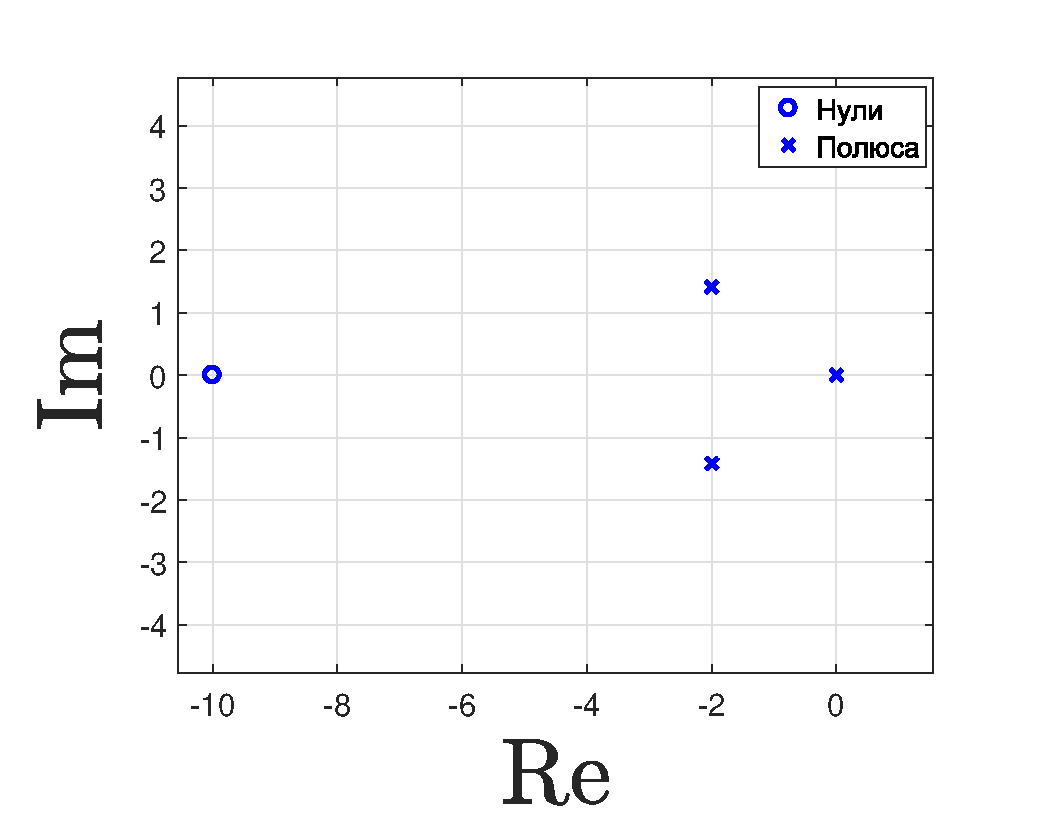
\includegraphics[width = 0.5\textwidth]{Open/pz}
		\caption{Нули и полюса разомкнутой системы}
		\label{openpz}
	\end{wrapfigure}
	
	Полюсами функции являются корни её характеристического уравнения её знаменателя, а нулями --- корни числителя. Таким образом
	\begin{align}
		&z_1 = -10, &p_1 &= 0,\\
		&p_2 = -2 + j\sqrt{2}, &p_3 &= -2 - j\sqrt{2},
	\end{align}
	где $z_1$ ноль функции, а $p_i, i = \overline{1,3}$ --- полюса.
	
	Для определения устойчивости системы обратимся к корневому критерию, в соответствии с которым система находится на нейтральной границе устойчивости, так как имеет чисто нулевой полюс и не имеет полюсов с положительной вещественной частью, что отчётливо видно на рисунке \ref{openpz}.
	
	Для определения определения логарифмических амплитудно-частотной и фазочастотной характеристик воспользуемся функцией \texttt{bode}. График, полученный в результате работы функции, приведён на рисунке \ref{openbode}.
	\begin{figure}[ht!]
		\centering
		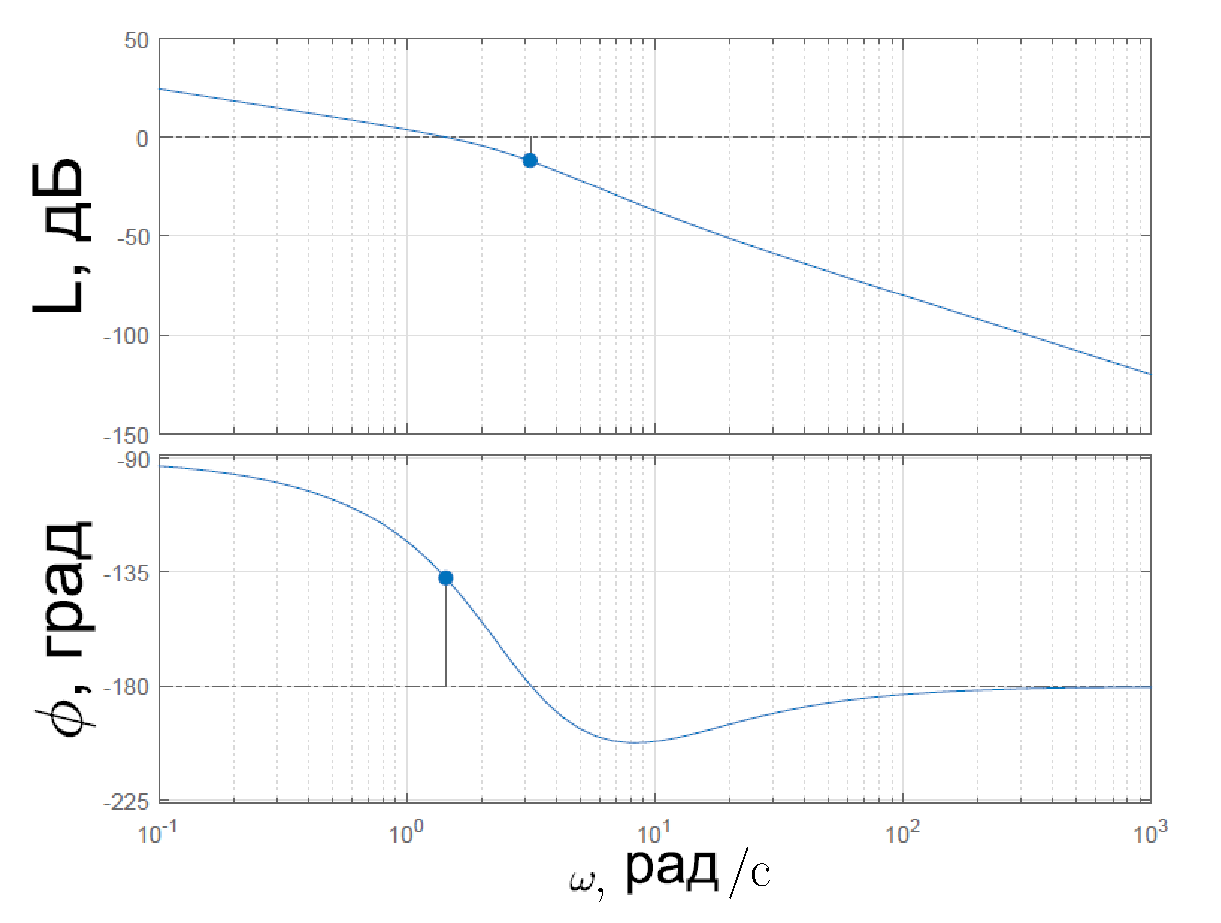
\includegraphics[height = 8.3cm]{Open/bode}
		\caption{Логарифмические характеристики разомкнутой системы}
		\label{openbode}
	\end{figure}
	
	При помощи функции \texttt{margin} определим запасы по амплитуде и частоте. Так же по полученным графикам определим значение частоты среза:
	\begin{align}
		&&\omega_\text{ср} = 1,45 \text{ рад/с}, &&A_\text{з} = 4, &&\varphi_\text{з} = 42,3^{\circ}.
	\end{align}
	
	При помощи функции \texttt{nyquistplot} построим амплитудно-фазовую частотную характеристику исследуемой системы. Результат работы функции приведён на рисунке \ref{opennyquist}.
	\begin{figure}[ht!]
		\centering
		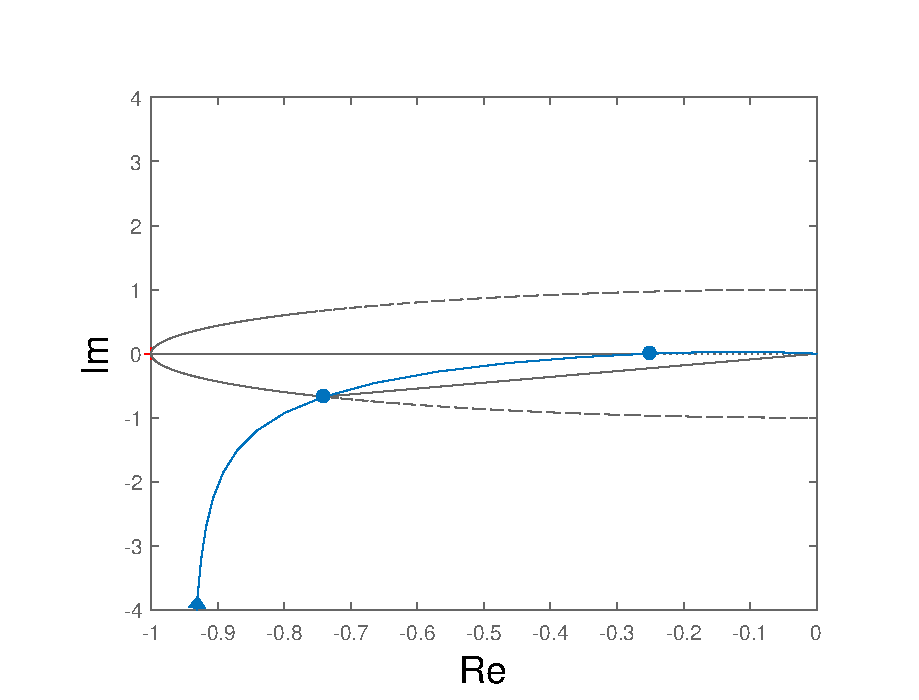
\includegraphics[width = \textwidth]{Open/nyquist}
		\caption{Амплитудно-фазовая частотная характеристика разомкнутой системы}
		\label{opennyquist}
	\end{figure}
	
	На приведённом графике видно, что АФЧХ системы не огибает точку (-1; 0), другими словами, фаза системы при частоте среза меньше $-180^{\circ}.$ Следовательно, система является устойчивой по критерию Найквиста.
	\clearpage
	{\centering
		\section{Анализ замкнутой системы}
	}
	Передаточная функция системы, замкнутой отрицательной обратной связью, в нашем случае будет иметь вид
	\begin{align}
		&&\Phi(s) = \frac{\displaystyle{\frac{s + 10}{s\cdot(s^2 + 4s + 6)}}}{1 + \displaystyle{\frac{s + 10}{s\cdot(s^2 + 4s + 6)}}\cdot K} = \frac{s + 10}{s^3 + 4s^2 + (6 + K)s + 10K}
	\end{align}
	
	Для определения влияния коэффициента $K$ на расположение полюсов замкнутой системы воспользуемся функцией \texttt{rlocus}. Полученный в результате график представлен на рисунке \ref{closedloc}.
	\begin{figure}[ht!]
		\centering
		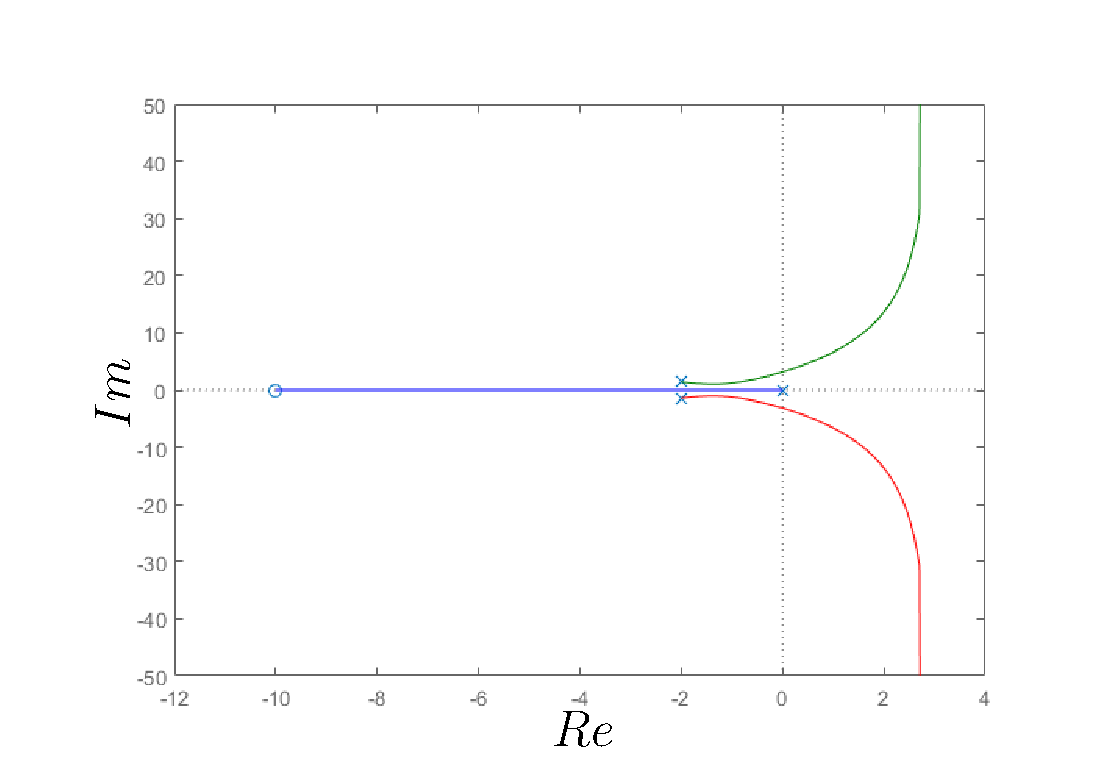
\includegraphics[width = 0.8\textwidth]{Closed/rlocus}
		\caption{Зависимость расположения полюсов замкнутой системы от коэффициента обратной связи}
		\label{closedloc}
	\end{figure}
	
	Для выбора коэффициента К воспользуемся корневым критерием устойчивости и составим матрицу Гурвница:
	\begin{align}
		&&\Gamma = \begin{bmatrix}
			4	&	10K	&	0	\\
			1	&	6+K	&	0	\\
			0	&	4	&	10K
		\end{bmatrix}.
	\end{align}
	Из неё видно, что при $K = 0$ система будет находиться на нейтральной границе устойчивости, при $K \in (0;4)$ --- устойчива, при $K = 4$ --- находиться на колебательной границе устойчивости и при $K > 4$ --- неустойчива.
	
	Выберем коэффициент обратной связи $K = 2,$ тогда передаточная функция замкнутой системы принимает вид
	\begin{align}
		&&\Phi(s) = \frac{s + 10}{s^3 + 4s^2 + 8s + 20}.
	\end{align}
	
	\begin{wrapfigure}{l}{0.5\textwidth}
		\centering
		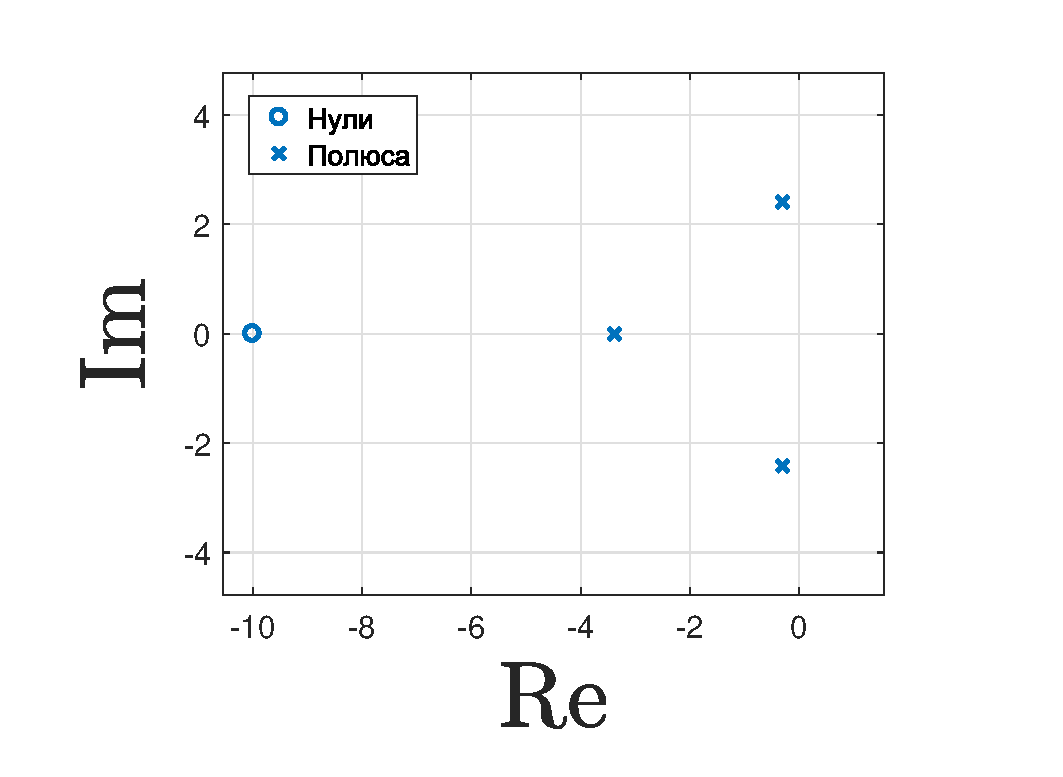
\includegraphics[width = 0.5\textwidth]{Closed/pz}
		\caption{Нули и полюса замкнутой системы}
		\label{closedpz}
	\end{wrapfigure}
	
	Найдём значения нулей и полюсов для замкнутой системы по графику, представленному на рисунке \ref{closedpz} и получим
	\begin{align}
		&z_1 = -10, &p_1 &= -3,38,\\
		&p_2 = -0,31 + j2,41, &p_3 & = -0,31 - j2,41.
	\end{align}
	
	Как можно заметить расположения полюсов не противоречат траекториям, отражённым на рисунке \ref{closedloc}, и система устойчива, так как не имеет корней с неотрицательной вещественной частью.
	
	Степенью устойчивости системы является наименьшее расстояние от комплексной оси до полюса системы. Таким образом в нашем случае степень устойчивости системы будет равна
	\begin{align}
		&&|\R e(p_2)| = |\R e(p_3)| = 0,31.
	\end{align}
	
	Воспользовавшись функциями \texttt{step} и \texttt{impulse} постоим графики переходной и весовой функций замкнутой системы. Результаты приведены на рисунке \ref{closedtpw}.
	\begin{figure}[ht!]
		\centering
		\begin{subfigure}[b]{0.49\textwidth}
			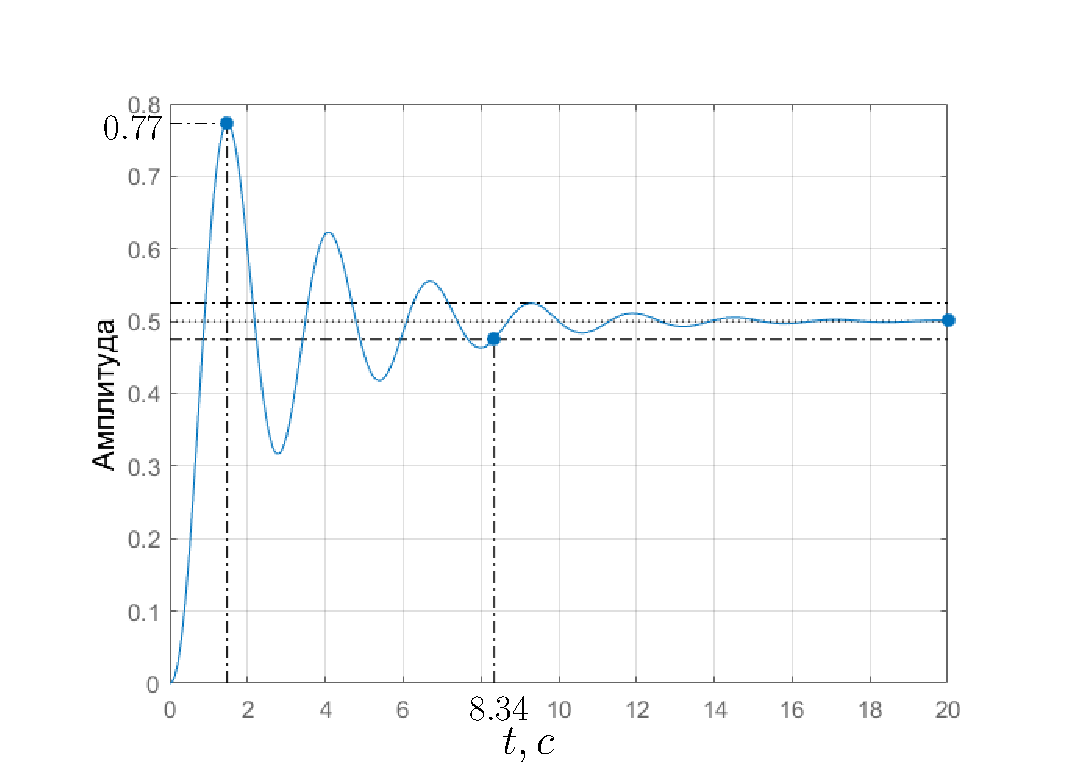
\includegraphics[width = \textwidth]{Closed/tp}
			\caption{Переходная функция}
		\end{subfigure}
		\hfill
		\begin{subfigure}[b]{0.49\textwidth}
			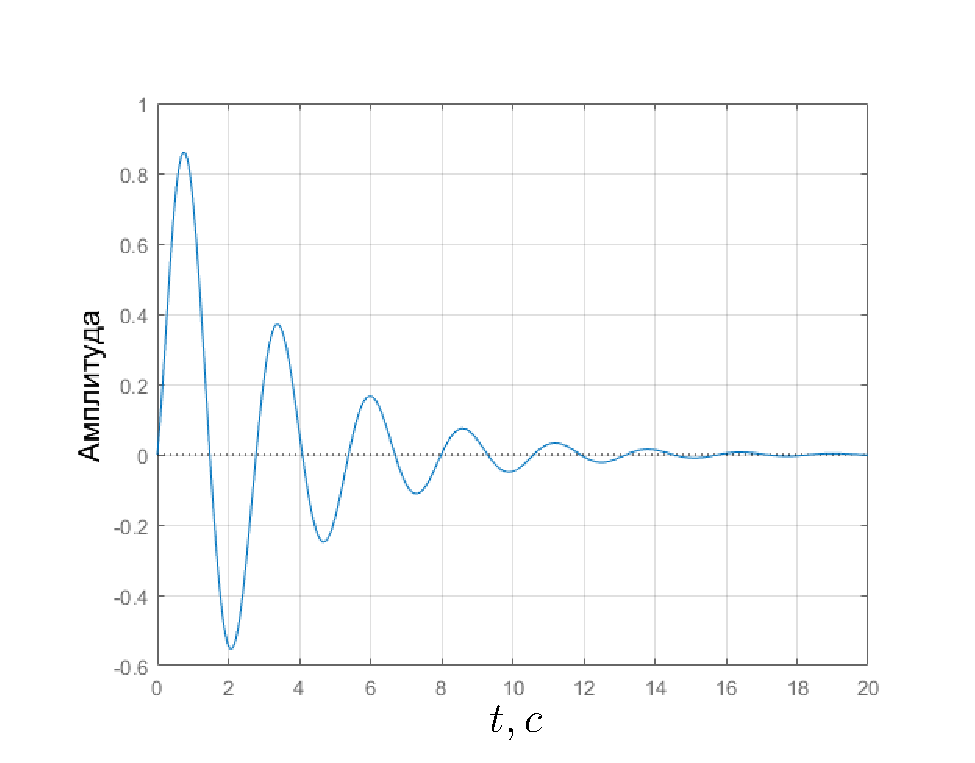
\includegraphics[width = \textwidth]{Closed/imp}
			\caption{Импульсная функция}
		\end{subfigure}
		\caption{Переходная и импульсная характеристики замкнутой системы}
		\label{closedtpw}
	\end{figure}
	
	По графику переходной функции определим величину перерегулирования, время переходного процесса и коэффициент затухания, так как наш процесс является колебательным:
	\begin{align}
		&&t_\text{п} = 8,34 c, &&\sigma = \frac{0,77 - 0,5}{0,5}\cdot100\% = 54\%, &&\beta = 0,063.
	\end{align}
	
	Представим замкнутую систему в форму Вход-Состояние-Выход. Для этого сначала получим дифференциальное уравнение, описывающее систему, проведя замену $s = \displaystyle{\frac{d}{dt}}.$
	\begin{align}
		&&\frac{d^3}{dt^3}y + 4\frac{d^2}{dt^2}y + 8\frac{d}{dt}y + 20y = \frac{d}{dt}u + 10u
	\end{align}
	\begin{align} \label{dereq}
		&&\dot{\ddot{y}} + 4\ddot{y} + 8\dot{y} + 20y = \dot{u} + 10u.
	\end{align}
	
	Записав выражение (\ref{dereq}) в форме Коши получим
	\begin{align} \label{koshi}
		&&\dot{x_3} = -4x_3 - 8x_2 - 20x_1 + u_2 + 10u_1,
	\end{align}
	где $x_1 = y, x_2 = \dot{y}, x_3 = \ddot{y}, u_1 = u, u_2 = \dot{u}$. Из уравнения (\ref{koshi}) составим модель Вход-Состояние-Выход в матричном виде в канонически управляемой форме:
	\begin{align}
		&&\begin{cases}
			\begin{bmatrix}
				\dot{x_1}\\
				\dot{x_2}\\
				\dot{x_3}
			\end{bmatrix} = \begin{bmatrix}
				0	&	1	&	0	\\
				0	&	0	&	1	\\
				-20	&	-8	&	-4				
			\end{bmatrix} \cdot \begin{bmatrix}
				x_1\\
				x_2\\
				x_3
			\end{bmatrix} + \begin{bmatrix}
				0\\
				0\\
				1
			\end{bmatrix} \cdot u\\
			y = \begin{bmatrix}
				10	&	1	&	0
			\end{bmatrix} \cdot \begin{bmatrix}
				x_1\\
				x_2\\
				x_3
			\end{bmatrix}
		\end{cases}.
	\end{align}
	
	Составим матрицу управляемости для полученной модели ВСВ.
	\begin{align}
		&&U_y = \begin{bmatrix}
			B	&	AB	&	A^2B
		\end{bmatrix} = \begin{bmatrix}
			0	&	0	&	0	\\
			0	&	1	&	-4	\\
			1	&	-4	&	8
		\end{bmatrix}, &&rank(U_y) = 3.
	\end{align}
	
	Так как ранг матрицы управляемости равен порядку системы, то система полностью управляема. Теперь составим матрицу наблюдаемости системы.
	\begin{align}
		&&U_\text{н} = \begin{bmatrix}
			C\\
			CA\\
			CA^2
		\end{bmatrix} = \begin{bmatrix}
			10	&	1	&	0	\\
			0	&	10	&	1	\\
			-20	&	-8	&	6
		\end{bmatrix}, &&rank(U_\text{н}) = 3.
	\end{align}
	Ранг полученной матрицы наблюдаемости равен порядку системы, следовательно, система является полностью наблюдаемой.
	\clearpage
	\section*{Вывод}
	При анализе разомкнутой системы на устойчивость следует придерживаться корневого критерия устойчивости, а не частотного, так как критерий Найквиста позволяет судить лишь об устойчивости замкнутой системы.
	
	При выборе коэффициента отрицательной обратной связи можно руководствоваться графиком, полученным в результате работы функции \texttt{rlocus} в среде Matlab. По нему легко определить расположение полюсов передаточной функции замкнутой системы при различных значениях коэффициента и, соответственно, оценить устойчивость системы по корневому критерию.
	
	В результате работы была получена устойчивая полностью наблюдаемая и полностью управляемая система с жесткой отрицательной обратной связью.
\end{document}